\documentclass[pdflatex,compress]{beamer}

%\usetheme[dark,framenumber,totalframenumber]{ElektroITK}
\usetheme[darktitle,framenumber,totalframenumber]{ElektroITK}

\usepackage{graphicx}

\title{FORENSIKA SUARA}
\subtitle{Konsep Dasar Sinyal dan Sistem Audio}

\author{Tim Dosen Pengampu}

\begin{document}

\maketitle

\section{Pendahuluan}

\begin{frame}
	\frametitle{Pendahuluan}
	\begin{itemize}
		\item Ilmu akustik dan audio engineering merupakan dasar dari audio forensik.
		\item Bukti audio forensik meliputi audio recording. \item Representasi dari bunyi yang dideteksi di udara oleh mikrofon, dikonversi menjadi tegangan, dan kemudian disimpan dalam suatu media.
		\item Rekaman audio bisa berupa analog maupun digital.
		\item Studi tentang akustik melibatkan prinsip fisika dari propagasi bunyi di udara.
	\end{itemize}
\end{frame}

\begin{frame}
	\frametitle{Pendahuluan}
	\begin{itemize}
		\item Untuk memahami dan menginterpretasikan rekaman forensik, perlu memahami konsep akustik sehingga bunyi yang dideteksi di dalam rekaman dapat dianalisis dan dikaitkan dengan karakteristik pemantulan (reflection), penyerapan (absorption), difraksi (diffraction), dan gema/dengung (reverberation) dari bunyi.
	\end{itemize}
\end{frame}

\section{Bunyi}

\begin{frame}
	\frametitle{Bunyi}
	\begin{itemize}
		\item Bunyi di udara merupakan hasil dari getaran.
		\item Partikel-partikel bergerak maju mundur dalam jarak pendek.
		\item 
	\end{itemize}
\end{frame}

\begin{frame}
	\begin{center}
		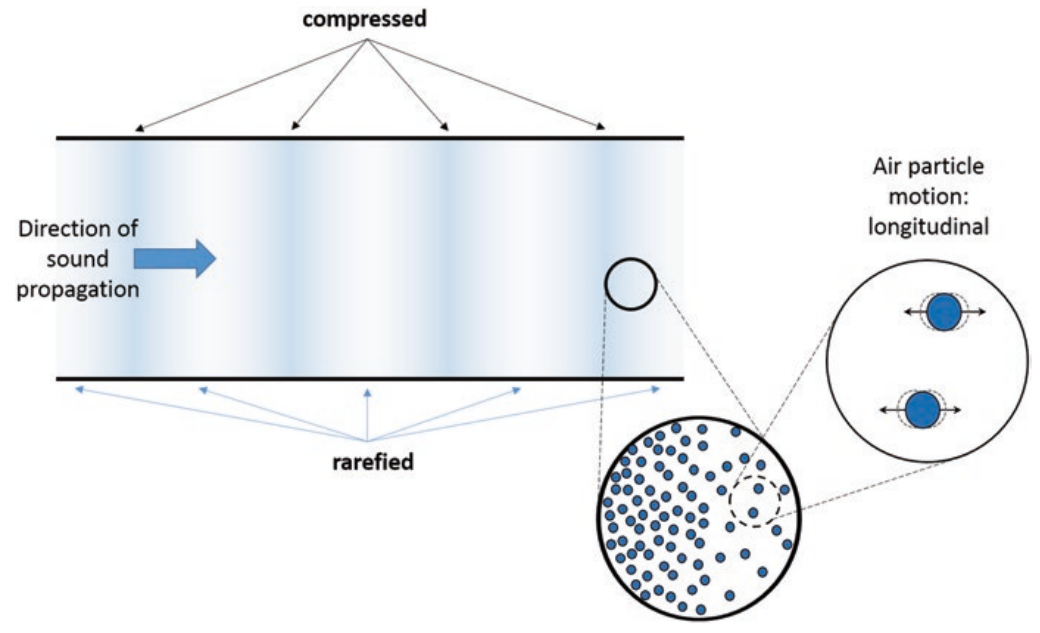
\includegraphics[width=0.7\linewidth]{img/img001}
	\end{center}
	
\end{frame}

\end{document}
